\documentclass{anstrans}
%%%%%%%%%%%%%%%%%%%%%%%%%%%%%%%%%%%
\title{Online reprocessing simulation for thorium-fueled molten salt breeder 
reactor}

\author{Andrei Rykhlevskii, Alexander Lindsay, Kathryn Huff}

\institute{
        Department of Nuclear, Plasma, and Radiological Engineering, University 
        of Illinois at Urbana-Champaign \break
        Urbana, IL
}

\email{andreir2@illinois.edu}

%%%% packages and definitions (optional)
\usepackage{graphicx} % allows inclusion of graphics
\usepackage{caption}  % allows center figures caption
\usepackage{booktabs} % nice rules (thick lines) for tables
\usepackage{microtype} % improves typography for PDF
\usepackage[section]{placeins}

\usepackage[acronym,toc]{glossaries}  % acronyms inclusion
%\newacronym{<++>}{<++>}{<++>}
\newacronym[longplural={metric tons of heavy metal}]{MTHM}{MTHM}{metric ton of heavy metal}
\newacronym{ABM}{ABM}{agent-based modeling}
\newacronym{ACDIS}{ACDIS}{Program in Arms Control \& Domestic and International Security}
\newacronym{AHTR}{AHTR}{Advanced High Temperature Reactor}
\newacronym{ANDRA}{ANDRA}{Agence Nationale pour la gestion des D\'echets RAdioactifs, the French National Agency for Radioactive Waste Management}
\newacronym{ANL}{ANL}{Argonne National Laboratory}
\newacronym{ANS}{ANS}{American Nuclear Society}
\newacronym{API}{API}{application programming interface}
\newacronym{ARE}{ARE}{Aircraft Reactor Experiment}
\newacronym{ARFC}{ARFC}{Advanced Reactors and Fuel Cycles}
\newacronym{ASME}{ASME}{American Society of Mechanical Engineers}
\newacronym{ATWS}{ATWS}{Anticipated Transient Without Scram}
\newacronym{BDBE}{BDBE}{Beyond Design Basis Event}
\newacronym{BIDS}{BIDS}{Berkeley Institute for Data Science}
\newacronym{CAFCA}{CAFCA}{ Code for Advanced Fuel Cycles Assessment }
\newacronym{CDTN}{CDTN}{Centro de Desenvolvimento da Tecnologia Nuclear}
\newacronym{CEA}{CEA}{Commissariat \`a l'\'Energie Atomique et aux \'Energies Alternatives}
\newacronym{CI}{CI}{continuous integration}
\newacronym{CNEN}{CNEN}{Comiss\~{a}o Nacional de Energia Nuclear}
\newacronym{CNERG}{CNERG}{Computational Nuclear Engineering Research Group}
\newacronym{COSI}{COSI}{Commelini-Sicard}
\newacronym{COTS}{COTS}{commercial, off-the-shelf}
\newacronym{CSNF}{CSNF}{commercial spent nuclear fuel}
\newacronym{CTAH}{CTAHs}{Coiled Tube Air Heaters}
\newacronym{CUBIT}{CUBIT}{CUBIT Geometry and Mesh Generation Toolkit}
\newacronym{CURIE}{CURIE}{Centralized Used Fuel Resource for Information Exchange}
\newacronym{DAG}{DAG}{directed acyclic graph}
\newacronym{DANESS}{DANESS}{Dynamic Analysis of Nuclear Energy System Strategies}
\newacronym{DBE}{DBE}{Design Basis Event}
\newacronym{DESAE}{DESAE}{Dynamic Analysis of Nuclear Energy Systems Strategies}
\newacronym{DHS}{DHS}{Department of Homeland Security}
\newacronym{DOE}{DOE}{Department of Energy}
\newacronym{DRACS}{DRACS}{Direct Reactor Auxiliary Cooling System}
\newacronym{DRE}{DRE}{dynamic resource exchange}
\newacronym{DSNF}{DSNF}{DOE spent nuclear fuel}
\newacronym{DYMOND}{DYMOND}{Dynamic Model of Nuclear Development }
\newacronym{EBS}{EBS}{Engineered Barrier System}
\newacronym{EDF}{EDF}{Électricité de France}
\newacronym{EDZ}{EDZ}{Excavation Disturbed Zone}
\newacronym{EIA}{EIA}{U.S. Energy Information Administration}
\newacronym{EPA}{EPA}{Environmental Protection Agency}
\newacronym{EPR}{EPR}{European Pressurized Reactors}
\newacronym{EP}{EP}{Engineering Physics}
\newacronym{EU}{EU}{European Union}
\newacronym{FCO}{FCO}{Fuel Cycle Options}
\newacronym{FCT}{FCT}{Fuel Cycle Technology}
\newacronym{FEHM}{FEHM}{Finite Element Heat and Mass Transfer}
\newacronym{FEPs}{FEPs}{Features, Events, and Processes}
\newacronym{FHR}{FHR}{Fluoride-Salt-Cooled High-Temperature Reactor}
\newacronym{FLiBe}{FLiBe}{Fluoride-Lithium-Beryllium}
\newacronym{FP}{FP}{Fission Products}
\newacronym{GDSE}{GDSE}{Generic Disposal System Environment}
\newacronym{GDSM}{GDSM}{Generic Disposal System Model}
\newacronym{GENIUSv1}{GENIUSv1}{Global Evaluation of Nuclear Infrastructure Utilization Scenarios, Version 1}
\newacronym{GENIUSv2}{GENIUSv2}{Global Evaluation of Nuclear Infrastructure Utilization Scenarios, Version 2}
\newacronym{GENIUS}{GENIUS}{Global Evaluation of Nuclear Infrastructure Utilization Scenarios}
\newacronym{GPAM}{GPAM}{Generic Performance Assessment Model}
\newacronym{GRSAC}{GRSAC}{Graphite Reactor Severe Accident Code}
\newacronym{GUI}{GUI}{graphical user interface}
\newacronym{HLW}{HLW}{high level waste}
\newacronym{HPC}{HPC}{high-performance computing}
\newacronym{HTC}{HTC}{high-throughput computing}
\newacronym{HTGR}{HTGR}{High Temperature Gas-Cooled Reactor}
\newacronym{IAEA}{IAEA}{International Atomic Energy Agency}
\newacronym{IEMA}{IEMA}{Illinois Emergency Mangament Agency}
\newacronym{IHLRWM}{IHLRWM}{International High Level Radioactive Waste Management}
\newacronym{INL}{INL}{Idaho National Laboratory}
\newacronym{IPRR1}{IRP-R1}{Instituto de Pesquisas Radioativas Reator 1}
\newacronym{IRP}{IRP}{Integrated Research Project}
\newacronym{ISFSI}{ISFSI}{Independent Spent Fuel Storage Installation}
\newacronym{ISRG}{ISRG}{Independent Student Research Group}
\newacronym{JFNK}{JFNK}{Jacobian-Free Newton Krylov}
\newacronym{LANL}{LANL}{Los Alamos National Laboratory}
\newacronym{LBNL}{LBNL}{Lawrence Berkeley National Laboratory}
\newacronym{LCOE}{LCOE}{levelized cost of electricity}
\newacronym{LDRD}{LDRD}{laboratory directed research and development}
\newacronym{LFR}{LFR}{Lead-Cooled Fast Reactor}
\newacronym{LLNL}{LLNL}{Lawrence Livermore National Laboratory}
\newacronym{LMFBR}{LMFBR}{Liquid Metal Fast Breeder Reactor}
\newacronym{LOFC}{LOFC}{Loss of Forced Cooling}
\newacronym{LOHS}{LOHS}{Loss of Heat Sink}
\newacronym{LOLA}{LOLA}{Loss of Large Area}
\newacronym{LP}{LP}{linear program}
\newacronym{LWR}{LWR}{Light Water Reactor}
\newacronym{MAGNOX}{MAGNOX}{Magnesium Alloy Graphie Moderated Gas Cooled Uranium Oxide Reactor}
\newacronym{MA}{MA}{minor actinide}
\newacronym{MCNP}{MCNP}{Monte Carlo N-Particle code}
\newacronym{MILP}{MILP}{mixed-integer linear program}
\newacronym{MIT}{MIT}{the Massachusetts Institute of Technology}
\newacronym{MOAB}{MOAB}{Mesh-Oriented datABase}
\newacronym{MOOSE}{MOOSE}{Multiphysics Object-Oriented Simulation Environment}
\newacronym{MOX}{MOX}{mixed oxide}
\newacronym{MSBR}{MSBR}{Molten Salt Breeder Reactor}
\newacronym{MSRE}{MSRE}{Molten Salt Reactor Experiment}
\newacronym{MSR}{MSR}{Molten Salt Reactor}
\newacronym{NAGRA}{NAGRA}{National Cooperative for the Disposal of Radioactive Waste}
\newacronym{NEAMS}{NEAMS}{Nuclear Engineering Advanced Modeling and Simulation}
\newacronym{NEUP}{NEUP}{Nuclear Energy University Programs}
\newacronym{NFCSim}{NFCSim}{Nuclear Fuel Cycle Simulator}
\newacronym{NGNP}{NGNP}{Next Generation Nuclear Plant}
\newacronym{NMWPC}{NMWPC}{Nuclear MW Per Capita}
\newacronym{NNSA}{NNSA}{National Nuclear Security Administration}
\newacronym{NPP}{NPP}{Nuclear Power Plant}
\newacronym{NPRE}{NPRE}{Department of Nuclear, Plasma, and Radiological Engineering}
\newacronym{NQA1}{NQA-1}{Nuclear Quality Assurance - 1}
\newacronym{NRC}{NRC}{Nuclear Regulatory Commission}
\newacronym{NSF}{NSF}{National Science Foundation}
\newacronym{NSSC}{NSSC}{Nuclear Science and Security Consortium}
\newacronym{NUWASTE}{NUWASTE}{Nuclear Waste Assessment System for Technical Evaluation}
\newacronym{NWF}{NWF}{Nuclear Waste Fund}
\newacronym{NWTRB}{NWTRB}{Nuclear Waste Technical Review Board}
\newacronym{OCRWM}{OCRWM}{Office of Civilian Radioactive Waste Management}
\newacronym{ORION}{ORION}{ORION}
\newacronym{ORNL}{ORNL}{Oak Ridge National Laboratory}
\newacronym{PARCS}{PARCS}{Purdue Advanced Reactor Core Simulator}
\newacronym{PBAHTR}{PB-AHTR}{Pebble Bed Advanced High Temperature Reactor}
\newacronym{PBFHR}{PB-FHR}{Pebble-Bed Fluoride-Salt-Cooled High-Temperature Reactor}
\newacronym{PEI}{PEI}{Peak Environmental Impact}
\newacronym{PH}{PRONGHORN}{PRONGHORN}
\newacronym{PRIS}{PRIS}{Power Reactor Information System}
\newacronym{PRKE}{PRKE}{Point Reactor Kinetics Equations}
\newacronym{PSPG}{PSPG}{Pressure-Stabilizing/Petrov-Galerkin}
\newacronym{PWAR}{PWAR}{Pratt and Whitney Aircraft Reactor}
\newacronym{PWR}{PWR}{Pressurized Water Reactor}
\newacronym{PyNE}{PyNE}{Python toolkit for Nuclear Engineering}
\newacronym{PyRK}{PyRK}{Python for Reactor Kinetics}
\newacronym{QA}{QA}{quality assurance}
\newacronym{RDD}{RD\&D}{Research Development and Demonstration}
\newacronym{RD}{R\&D}{Research and Development}
\newacronym{RELAP}{RELAP}{Reactor Excursion and Leak Analysis Program}
\newacronym{RIA}{RIA}{Reactivity Insertion Accident}
\newacronym{RIF}{RIF}{Region-Institution-Facility}
\newacronym{SFR}{SFR}{Sodium-Cooled Fast Reactor}
\newacronym{SINDAG}{SINDA{\textbackslash}G}{Systems Improved Numerical Differencing Analyzer $\backslash$ Gaski}
\newacronym{SKB}{SKB}{Svensk K\"{a}rnbr\"{a}nslehantering AB}
\newacronym{SNF}{SNF}{spent nuclear fuel}
\newacronym{SNL}{SNL}{Sandia National Laboratory}
\newacronym{STC}{STC}{specific temperature change}
\newacronym{SUPG}{SUPG}{Streamline-Upwind/Petrov-Galerkin}
\newacronym{SWF}{SWF}{Separations and Waste Forms}
\newacronym{SWU}{SWU}{Separative Work Unit}
\newacronym{TRIGA}{TRIGA}{Training Research Isotope General Atomic}
\newacronym{TRISO}{TRISO}{Tristructural Isotropic}
\newacronym{TSM}{TSM}{Total System Model}
\newacronym{TSPA}{TSPA}{Total System Performance Assessment for the Yucca Mountain License Application}
\newacronym{ThOX}{ThOX}{thorium oxide}
\newacronym{UFD}{UFD}{Used Fuel Disposition}
\newacronym{UML}{UML}{Unified Modeling Language}
\newacronym{UOX}{UOX}{uranium oxide}
\newacronym{UQ}{UQ}{uncertainty quantification}
\newacronym{US}{US}{United States}
\newacronym{UW}{UW}{University of Wisconsin}
\newacronym{VISION}{VISION}{the Verifiable Fuel Cycle Simulation Model}
\newacronym{VVER}{VVER}{Voda-Vodyanoi Energetichesky Reaktor (Russian Pressurized Water Reactor)}
\newacronym{VV}{V\&V}{verification and validation}
\newacronym{WIPP}{WIPP}{Waste Isolation Pilot Plant}
\newacronym{YMR}{YMR}{Yucca Mountain Repository Site}


\usepackage{tabularx} % for nice wrapping of table text

\makeglossaries

\graphicspath{{figures/}}

\newcommand{\SN}{S$_N$}
\renewcommand{\vec}[1]{\bm{#1}} %vector is bold italic
\newcommand{\vd}{\bm{\cdot}} % slightly bold vector dot
\newcommand{\grad}{\vec{\nabla}} % gradient
\newcommand{\ud}{\mathop{}\!\mathrm{d}} % upright derivative symbol

\begin{document}
%%%%%%%%%%%%%%%%%%%%%%%%%%%%%%%%%%%%%%%%%%%%%%%%%%%%%%%%%%%%%%%%%%%%%%%%%%%%%%%%
\section{Introduction}
The thermal spectrum \gls{MSR} is an advanced type of reactor that consists of 
constantly circulating liquid fuel (i.e., mixture of $LiF-BeF_2-ThF_4-UF_4$ or 
$LiF-BeF_2-ZrF_4-UF_4$) and solid graphite moderator structures. This liquid 
fuel form leads to immediate advantages over traditional, 
solid-fueled, reactors. The molten-salt carrier with dissolved 
fissile and/or fertile material allows for online refuelling and 
reprocessing. Thus, \glspl{MSR} can potentially operate years without shutdown, 
achieving maximum fuel utilization and outstanding neutron economy 
\cite{leblanc_molten_2010}. Moreover, this type of fuel does not need 
complex fabrication since the fissile material could be transported from any 
enrichment plant to the \gls{NPP} in the form 
of uranium hexafluoride ($UF_6$).  Additionally, \glspl{MSR} have a high level 
of inherent safety due to their characteristically 
strong negative temperature coefficient of reactivity, near-atmospheric 
pressure in the primary loop, stable coolant, passive decay heat cooling, and 
small excess reactivity \cite{elsheikh_safety_2013}.

The thorium-fueled \gls{MSBR} was developed in the early 1970s by \gls{ORNL} 
specifically to realize the promise of the thorium fuel cycle which allows the 
use of natural thorium instead of enriched uranium as the fertile element. 
Thorium breeds the fissile $^{233}U$ and avoids uranium enrichment 
\cite{robertson_conceptual_1971}. In the matter of nuclear fuel cycle, the 
thorium cycle produces a reduced quantity of plutonium and \glspl{MA} 
compared to the traditional uranium fuel cycle. Consequently, it may 
significantly increase proliferation resistance when the \gls{MSR} operates in the 
breeder regime. The \glspl{MSR} also could be employed as a converter reactor for 
transmutation or spent fuel from current \glspl{LWR}.

Recently, interest in \glspl{MSR} has resurged, with multiple new companies 
pursuing commercialization of \gls{MSR} designs\footnote{Examples include both 
liquid-fueled molten salt designs from Transatomic, Terrapower, Terrestrial, 
and Thorcon.}.
To further develop these \gls{MSR} concepts, particularly with respect to their  
strategies for online reprocessing and refueling, computational analysis methods capturing
their unique reactor physics and process chemistry are needed.
However, most contemporary nuclear reactor physics software is unable to 
perform depletion calculations in an online reprocessing 
regime. Powers \emph{et al.} suggested a novel method for conducting 
depletion simulations for \gls{MSR}. This suggested method takes into account 
fuel salt composition changes due to online 
reprocessing and refueling based on the deterministic computer code NEWT in 
SCALE \cite{powers_new_2013}. This approach was later used by Jeong \emph{et 
al.} to find an equilibrium fuel composition for the \gls{MSBR} and was 
validated with an \gls{MCNP}/CINDER90 model \cite{jeong_equilibrium_2016}. 

The current paper presents a single-cell model developed using the
continuous-energy Serpent 2 Monte Carlo reactor physics software. It was 
employed to establish a Serpent-based method for finding the equilibrium core composition and 
core depletion of the \gls{MSBR}.
All calculations presented in this paper were performed using the Serpent 2 
code version 2.1.29 with ENDF/B-VII.0
nuclear data \cite{leppanen_serpent_2012,chadwick_endf/b-vii.0:_2006}. Serpent 
2 is an improvement upon Serpent 1, and contains a complete 
redesign of memory management using hybrid OpenMP + MPI parallelization.  This 
hybrid parallelization is important in depletion calculations using computer 
clusters with multiple cores \cite{leppanen_serpent_2015}. This work used the 
built-in Serpent 2 depletion capabilities and its built-in online reprocessing 
subroutine. Another feature of the \gls{MSBR}, its circulating liquid fuel and 
corresponding delayed neutron precursor drift, is not treated here.

%%%%%%%%%%%%%%%%%%%%%%%%%%%%%%%%%%%%%%%%%%%%%%%%%%%%%%%%%%%%%%%%%%%%%%%%%%%%%%%%
\section{Description of the actual work}
The \gls{MSBR} is a thermal spectrum reactor. The reactor vessel has a diameter of 
$680 cm$ and a height of $610 cm$. It contains a molten fluoride fuel-salt mixture 
which performs two functions: to generate heat in the moderated region and to 
transport heat energy from the core to primary heat exchanger using the primary 
salt pump. The vessel also contains graphite blocks for neutron moderation and 
reflection. The lithium in the fuel-salt solution is enriched to 99.995\% 
$^7$Li because $^6$Li is a very strong neutron poison and becomes tritium upon 
neutron bombardment. In this study, the 0.005\% atomic fraction of $^6$Li has 
been taken into account because even such a small amount of isotope with very 
high absorption cross section can significantly impact the neutron flux energy 
distribution and, consequently, depletion calculation results. 
Table~\ref{tab:data} is the summary of the major \gls{MSBR} parameters used by 
this model \cite{robertson_conceptual_1971}. 

%%%%%%%%%%%%%%%%%%%%%%%%%%%%%%%%%%%%%%%%
\captionsetup[table]{
        labelsep = newline,
        name = TABLE, justification=justified,
        singlelinecheck=false,%%%%%%% a single line is centered by default
        labelsep=colon,%%%%%%
skip = \medskipamount}
\begin{table}[h!]
        %\centering
        %\begin{tabular}{p{0.46\linewidth} p{0.50\linewidth}} \toprule
        \begin{tabularx}{\linewidth}{l X} \toprule 
                Thermal capacity of reactor           & 2250 MW(t)
                \\ \midrule
                %Net electrical output                 & 1000 MW(e) \\ \midrule
                %Net thermal efficiency        & 44.4\%
                %\\ \midrule
                Salt volume fraction in central core zone     & 0.132
                \\ \midrule
                Salt volume fraction in outer core zone       & 0.37
                \\ \midrule
                Fuel-salt inventory (Zone I)                  & 8.2 m$^3$	
                \\ \midrule
                Fuel-salt inventory (Zone II)                 & 10.8 m$^3$	
                \\ \midrule
                Fuel salt components                  & 
                LiF-BeF$_2$-ThF$_4$-$^{233}$UF$_4$-$^{239}$PuF$_3$	\\ 
                \midrule
                Fuel salt composition                 & 
                71.767-16-12-0.232-0.0006 mole\%
                \\
                \bottomrule
        \end{tabularx}
        \caption{Summary of principal data for MSBR.}
        \label{tab:data}
\end{table}
%%%%%%%%%%%%%%%%%%%%%%%%%%%%%%%%%%%%%%%%%%%%%%%%

The \gls{MSBR} core consists of two different zones. The central 
zone, Zone I, in which 13.2\% of the volume is fuel salt and 86.8\% graphite. 
Zone I composed of 1320 graphite cells, 2 graphite control rods, and 
2 safety rods consisting of boron carbide clad. The under-moderated zone, Zone 
II, with 37\% fuel salt, and radial reflector, surrounds the Zone I core region 
and serves to diminish neutron leakage. In this work, 
only a Zone I element with a $3.42138 cm$ diameter central fuel channel and molten-salt 
fuel volume fraction of 0.132 was considered. Figure~\ref{fig:zoneI} shows the 
geometry of the unit cell model. The boundary condition of the unit cell is 
periodic. The density of the fuel salt is $3.3304 g/cm^3$ and the graphite density is 
$1.843 g/cm^3$. The temperature of fuel and graphite is fixed at 908K for the whole 
reprocessing cycle \cite{robertson_conceptual_1971}.

\begin{figure}[htbp!] % replace 't' with 'b' to force it to be on the bottom
        \centering
        \includegraphics[width=0.90\linewidth]{zone_I_mesh.png}
        \caption{MSBR unit cell of Zone I geometry.}
        \label{fig:zoneI}
\end{figure}

\FloatBarrier
\subsection{Online reprocessing method}

Currently, researchers 
investigating the \glspl{MSR} 
typically develop custom supporting tools and scripts to simulate 
online reprocessing and refueling. Most utilize stochastic (i.e. 
\gls{MCNP}) or deterministic (i.e. SCALE) methods for depletion and supplement 
these with custom Python scripts to capture the impacts of reprocessing 
\cite{jeong_equilibrium_2016,park_whole_2015}. Serpent 2 is the 
first commonly used monte carlo software to support continuous material 
reprocessing. It does so by allowing the user to 
define multiple material flows into and out of the fuel. This work applies this 
Serpent 2 feature to the \gls{MSBR}. 

The \gls{MSBR} has the capability to remove all poisons
(e.g. 
$^{135}$Xe), noble metals, and gases (e.g. $^{75}$Se, $^{85}$Kr) 
every 20 seconds. The $^{232}$Th in the fuel absorbs thermal 
neutrons and produces $^{233}$Pa which then decay into the fissile $^{233}$U. 
Protactinium presents a challenge, since it has a large absorption cross section in the thermal 
energy spectrum. Accordingly, $^{233}$Pa is continuously removed from the fuel salt 
into a protactinium decay tank and allowing $^{233}$Pa to decay to $^{233}$U without 
poisoning the reactor. The reactor reprocessing system is designed to separate 
$^{233}$Pa from the molten-salt fuel over 3 days, hold it while $^{233}$Pa 
decays into $^{233}$U, and return it back to the primary loop. This feature allows the reactor to 
avoid neutron losses to protactinium, keeps fission products to a very low level, and 
increases the efficiency of $^{233}$U breeding \cite{robertson_conceptual_1971}.

Since removal rates vary among nuclides in this reactor concept, the Serpent 2 
reprocessing method is unable to capture the desired reprocessing strategy. 
The removal rates also dictate the necessary resolution of depletion 
calculations. If the depletion time intervals are 
very short an enormous number of depletion steps are required to
obtain the equilibrium composition. On the other hand, if the depletion 
calculation time interval is too long, serious impacts of short lived fission 
products are not captured in a manner that is faithful \gls{MSBR} conceptual design. 
To compromise, the time interval for depletion calculations in this model was selected 
as 3 days to correlate with the removal interval of $^{233}$Pa and Thorium was 
continuously added to maintain the initial mass fraction of $^{232}$ThF$_4$.

%%%%%%%%%%%%%%%%%%%%%%%%%%%%%%%%%%%%%%%%%%%%%%%%%%%%%%%%%%%%%%%%%%%%%%%%%%%%%%%%
\section{Results and Analysis}

Using the methodology described previously, the \gls{MSBR} unit cell depletion 
analysis was performed to find equilibrium core conditions. Calculation results reported 
in this section include multiplication factor, neutron flux energy 
spectrum, and atomic density of major isotopes.

\subsection{Equilibrium state analysis}

This analysis models a single representative unit cell rather than the whole 
\gls{MSBR} core. Consequently, it does not take into consideration different 
fuel-moderator volume ratios for Zone I, Zone II, the annulus, and the reflector. The 
initial multiplication factor during depletion calculation is selected for 
a state with fully withdrawn control rods, which gives 
considerable excess reactivity in the beginning of the cycle (approximately 5000 pcm). 
Standard deviation for these calculations is approximately 100 pcm.

\begin{figure}[htbp!] % replace 't' with 'b' to force it to be on the bottom
        \centering
        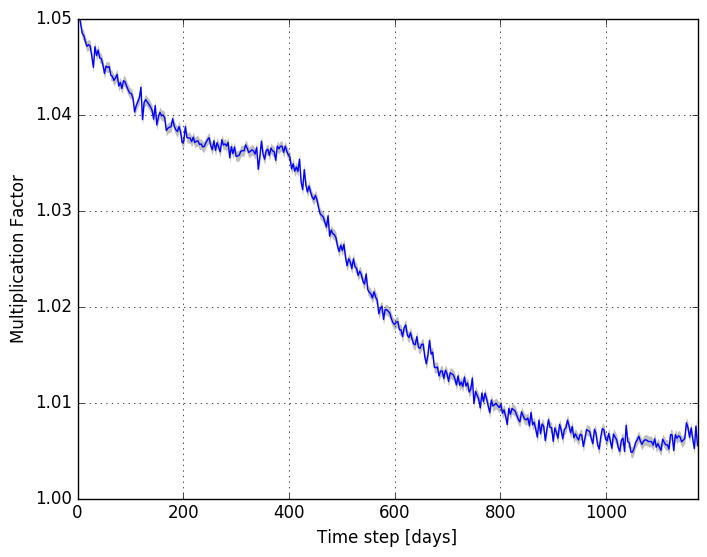
\includegraphics[width=1.03\linewidth]{keff.png}
        \caption{Infinite multiplication factor during a 4-years depletion 
        simulation.}
        \label{fig:keff}
\end{figure}

\FloatBarrier

Figure~\ref{fig:keff} shows the infinite multiplication factor for 4-year 
reprocessing cycle calculated by Serpent 2 with ENDF/B-VII.0 nuclear data. A 
significant standard deviation (100 pcm) causes the multiplication factor 
fluctuations visible in this plot.  Protactinium-233 continuously removing into 
the tank for protactinium decay.  $^{233}$Pa has a half-life of 27 days and 
beta decays into $^{233}$U which as fresh fuel goes back to the reactor core. 
The infinite multiplication factor decreases first 400 days of depletion due to 
strong absorbers (e.g. $^{233}$Th, $^{234}$U) accumulation which causes 
relatively high fuel ($^{233}$U) refill inflow to keep reactor critical. During 
reactor operation producing fissile materials other than $^{233}$U in the core 
(e.g. $^{235}$U, $^{239}$Pu) which makes it possible to decrease fresh fuel 
refill rate after ~1 year of operation.

\begin{figure}[htbp!] % replace 't' with 'b' to force it to be on the bottom
        \centering
        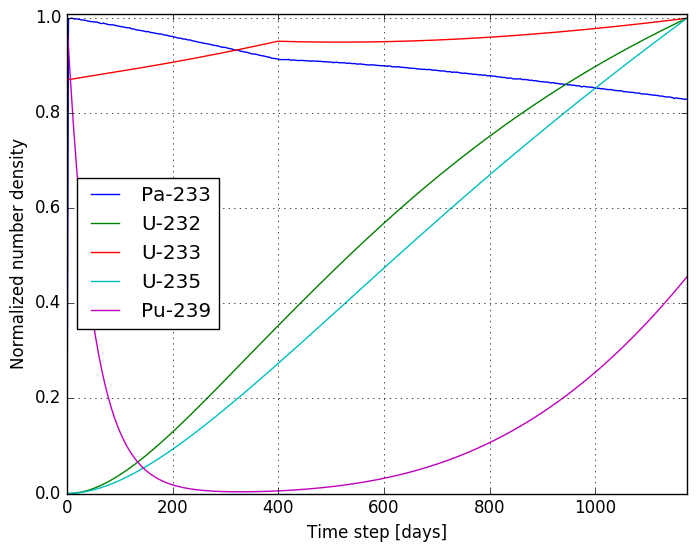
\includegraphics[width=1.03\linewidth]{fuel_composition.png}
        \caption{Normalized number density of major isotopes during 4 years of 
        depletion.}
        \label{fig:compos}
\end{figure}

\FloatBarrier

The analysis of the fuel salt composition variation gives clearer information 
about the equilibrium core state. Figure~\ref{fig:compos} shows the normalized 
number density of isotopes influential to core 
neutronics at the beginning of each depletion time interval. The number density 
of protactinium is very low (less than $10^{16}$1/cm$^3$) but some small amount 
of it is produced during the 3-day reprocessing period. In this assessment, the multiplication 
factor stabilizes after approximately 950 days. 
Figure~\ref{fig:rates} represents the rates of online reprocessing material flows
flows over the 4-year depletion calculation. 
%%%%%%%%%%%%%%%%%%%%%%%%%%%%%%%%%%%%%%%%
%\captionsetup[table]{
%  labelsep = newline,
%  name = TABLE, justification=justified,
%  singlelinecheck=false,%%%%%%% a single line is centered by default
%  labelsep=colon,%%%%%%
%  skip = \medskipamount}
%\begin{table}[h!]
%\centering
%\begin{tabular}{p{0.25\linewidth} p{0.3\linewidth} p{0.3\linewidth}} \toprule
%      Isotope & First 400 days     & After 400 days          
%\\ \midrule
%$^{232}$Th  & 3.704$\times10^{12}$ & 3.086$\times10^{12}$
%\\ \midrule
%$^{233}$Pa  & 3.704$\times10^{12}$ & 3.086$\times10^{12}$
%\\ \midrule
%$^{233}$U  & $1.05134\pm0.00116$ & $1.00736$
%\\
%\bottomrule
%\end{tabular}
%  \caption{Materials flows rates during \gls{MSBR} online reprocessing 
%  [1/s*cm$^3$].}
%  \label{tab:rates}
%\end{table}
%%%%%%%%%%%%%%%%%%%%%%%%%%%%%%%%%%%%%%%%%%%%%%%%%%%%%%%%%%%%%%%%%%%%%%%%%%%%%%%%
\begin{figure}[htbp!] % replace 't' with 'b' to force it to be on the bottom
        \centering
        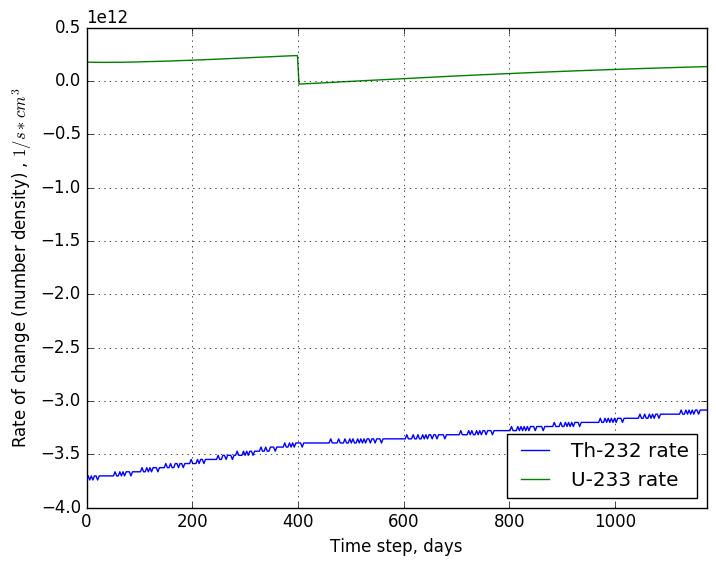
\includegraphics[width=1.03\linewidth]{rates_fuel.png}
        \caption{Materials flows rates during online reprocessing.}
        \label{fig:rates}
\end{figure}
In Figure~\ref{fig:rates} we can see that, to keep the reactor critical, a higher $^{233}$U 
flow rate from the protactinium decay tank was required for first 400 days of 
operation. After that, the $^{233}$U flow rate can be reduced. The $^{232}$Th 
rate slightly decreases over 4 years of operation due to other than $^{233}$U 
fissile materials accumulation.

\begin{figure}[htbp!] % replace 't' with 'b' to force it to be on the bottom
        \centering
        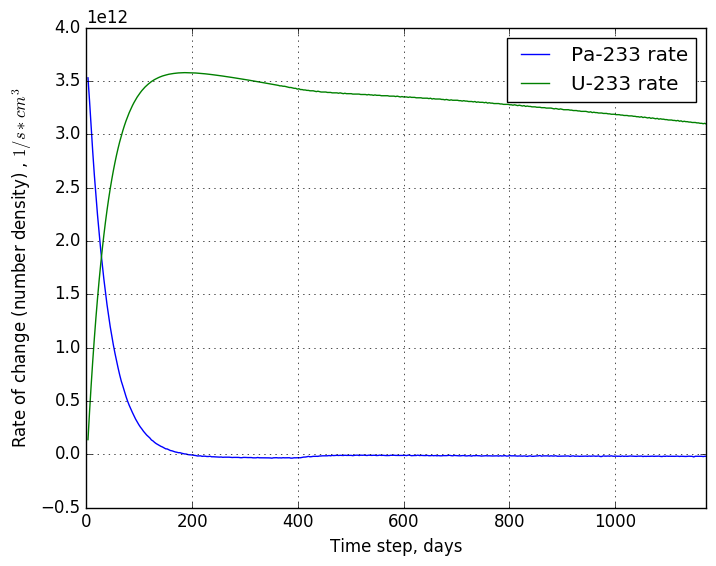
\includegraphics[width=1.03\linewidth]{rates_outflow.png}
        \caption{Materials flows rates for the protactinium decay tank during 
        \gls{MSBR} online reprocessing.}
        \label{fig:outflow}
\end{figure}
As shown in Figure~\ref{fig:outflow}, the tank for protactinium decay 
accumulates $^{233}$Pa for approximately 200 days. Fresh $^{233}$U fuel flow is 
also established after 200 days. Uranium produced in the tank by protactinium 
decay is separated by circulation of the salt through a flourinator. The fully 
processed molten salt, on its way back to the primary loop, has uranium added 
at the rate required to maintain or adjust the fissile material concentration 
and, hence, the reactivity, in the reactor core as desired.

\subsection{Neutron spectrum}

Figure~\ref{fig:spectrum} represents the normalized neutron flux distribution 
of the initial and the equilibrium core compositions. The spectrum for the 
equilibrium state is harder than the initial state due to heavy fission 
products.  
\begin{figure}[htbp!] % replace 't' with 'b' to force it to be on the bottom
        \centering
        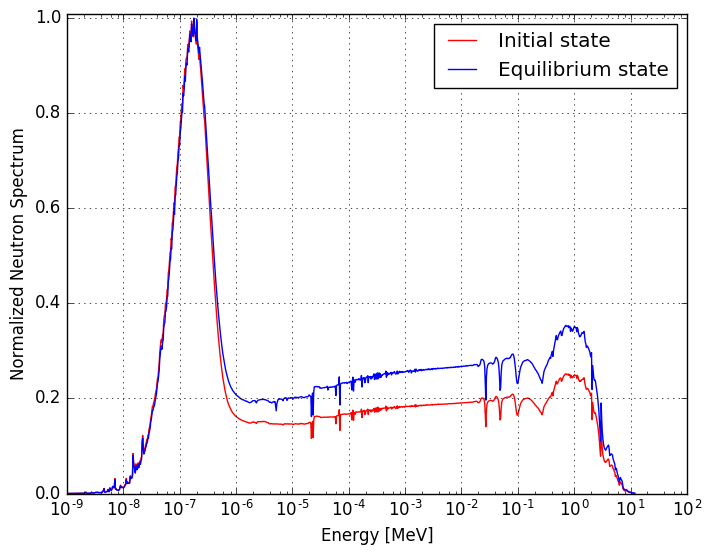
\includegraphics[width=1.04\linewidth]{spectrum.png}
        \caption{Normalized neutron energy spectrum for initial and equilibrium 
        composition.}
        \label{fig:spectrum}
\end{figure}

\FloatBarrier 

In this work, only the Zone I unit cell, where the fuel salt volume fraction is 
13.2\%, was considered. The neutron spectrum for Zone II cell, where the fuel 
salt volume fraction is 37\% is expected to be harder and the peak in thermal 
energy region is predicted to be much 
lower. To obtain a high-fidelity neutron energy spectrum, a full-core \gls{MSBR}
analysis is required.
%%%%%%%%%%%%%%%%%%%%%%%%%%%%%%%%%%%%%%%%%%%%%%%%%%%%%%%%%%%%%%%%%%%%%%%%%%%%%%%%
\section{Conclusions}
The depletion calculation of the \gls{MSBR} unit cell model for finding the 
equilibrium states was performed using the Serpent 2 Monte Carlo code to 
simulate simplified case of the online reprocessing and refueling to find 
equilibrium material composition. When running depletion calculation, the 
fission products are removed and fertile/fissile materials are added to fuel 
salt every 3 days. The important MSR feature, online reprocessing \& refueling 
is implemented in the Serpent 2 material burnup routine. The results of this 
study indicate that from the depletion calculation the multiplication factor 
slowly decreases and reaches to the equilibrium state. The most obvious finding 
to emerge from the analysis of initial and equilibrium materials composition is 
that neutron energy spectrum is harder for equilibrium state because 
significant amount of heavy fission products were accumulated in the \gls{MSBR} 
core.

These results are contrary with those of Jeong and Park (2016) who suggested 
two different unit cell models and uses \gls{MCNP} with Python-script to 
simulate \gls{MSBR} online reprocessing to find equilibrium composition. This 
inconsistency may be due to different fuel fraction in the unit cell (Jeong and 
Park selected 20.6\% salt fraction). To obtain better results for this online 
reprocessing simulation, many future efforts are planned. First, a depletion 
simulation will be performed using a  full-core, three-dimensional, high-fidelity 
model of \gls{MSBR} that has been developed in Serpent 2. In this case, different 
fuel-moderator volume ratios for the reactor Zone I, Zone II, annulus, 
and reflectors will be taken into account to find accurate multiplication factor, 
neutron spectrum and, hence, depleted composition. Secondly, an additional Serpent 
2 flow control system subroutine should be developed to simulate adjusting 
material flows (e.g. rate of removing $^{233}$Pa from the salt and adding 
fissile $^{233}$U from the tank for protactinium decay) depending upon the 
instantaneous reactivity value, which is a more promising reactivity control method than moving 
control rods. Finally, the temperature effect of reactivity for both 
fuel salt and graphite should be calculated to find optimal effective 
multiplication factor range. 

%%%%%%%%%%%%%%%%%%%%%%%%%%%%%%%%%%%%%%%%%%%%%%%%%%%%%%%%%%%%%%%%%%%%%%%%%%%%%%%%
\bibliographystyle{ans}
\bibliography{bibliography}
\end{document}

